\documentclass[10pt,conference]{IEEEtran}
\usepackage{amsmath}
\usepackage{booktabs}
\usepackage{graphicx}
\usepackage{url}
\usepackage{hyperref}
\usepackage{algorithm}
\usepackage{algpseudocode}

\title{Focus RNG: A Reproducible CPU/GPU/QPU Benchmarking Framework for Runtime-Resource Trade-off Analysis}

\author{\IEEEauthorblockN{Anonymous for Review}}

\begin{document}
\maketitle

\begin{abstract}
This paper presents a repository-backed benchmarking framework for comparing random number generation (RNG) workloads across CPU, GPU, and QPU backends. The implementation unifies execution paths in a single interface, adds explicit backend provenance (\texttt{backend\_type}, fallback flags), and exports reproducible artifacts (JSON/CSV/Markdown/figures). The main experiment uses warmup runs and repeated trials with 95\% confidence intervals over workload sizes $N=\{64,128,256,512,1024\}$. In the current environment, CUDA is unavailable, so all GPU runs execute in CPU fallback mode and are excluded from primary analysis. CPU mean time is $3.97\times10^{-5}$ s while QPU-simulator mean time is $0.129955$ s. Real GPU acceleration and real QPU-hardware advantage are not supported by current repository evidence.
\end{abstract}

\section{Introduction}
Cross-architecture benchmarking often conflates true hardware execution with fallback execution. This repository addresses that gap for RNG workloads by explicitly tagging backend provenance and separating analyzed versus excluded runs.

The contribution is practical: a reproducible benchmarking pipeline rather than a novel quantum algorithm.

\section{Related Work}
CPU/GPU pseudo-random generation benchmarking has prior coverage in applied literature~\cite{askar2021gpu}. QRNG workflows on cloud superconducting platforms have been explored~\cite{li2021cloudqrng}, and certified quantum randomness has been reported at larger scales~\cite{nature2025certified}. This repository differs by emphasizing execution provenance, fallback filtering, and reproducibility artifacts.

\section{Methodology}
\subsection{Task Definition}
For each workload size $N$, generate $N$ integer samples in range $[0,2^q-1]$, where $q$ is either fixed or $\lceil\log_2 N\rceil$.

\subsection{Complexity Framing}
The codebase uses expected complexity framing:
\begin{itemize}
\item CPU: $O(N)$
\item GPU: approximately $O(N/P)$ with effective parallelism $P$
\item QPU resource width in \texttt{logn} mode: $q\approx\lceil\log_2 N\rceil$
\end{itemize}

\subsection{Statistics}
95\% confidence intervals use normal approximation:
\begin{equation}
\mathrm{CI}_{95\%}=\bar{x}\pm1.96\cdot\frac{s}{\sqrt{n}}.
\end{equation}
Speedup from mean timings:
\begin{equation}
\mathrm{Speedup}_{A\leftarrow B}(N)=\frac{T_A(N)}{T_B(N)}.
\end{equation}
Where sample sizes permit, Welch's two-sample t-tests are computed for pairwise timing comparisons (see \texttt{paper/tables/table\_significance\_welch\_ttest.csv}).

\section{System Architecture}
\begin{figure}[t]
  \centering
  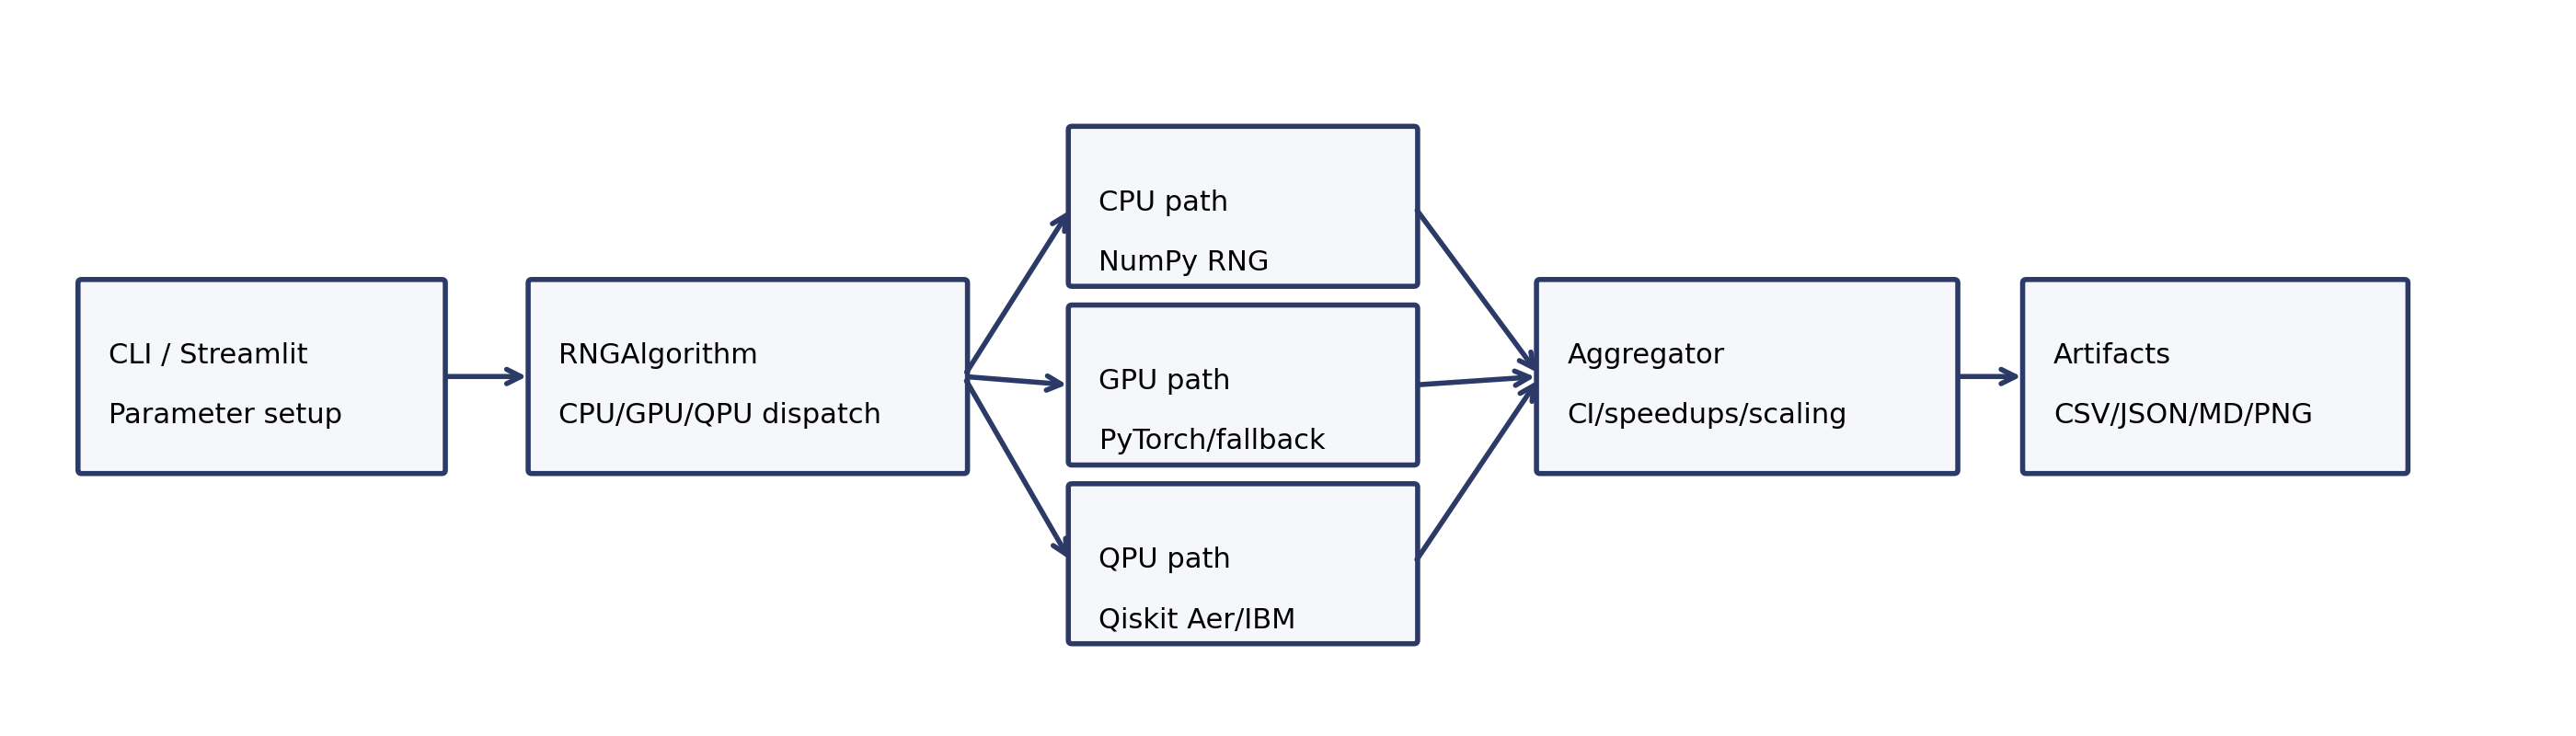
\includegraphics[width=0.98\columnwidth]{figures/fig_pipeline_architecture.png}
  \caption{Benchmark pipeline from parameter configuration to artifact export.}
  \label{fig:pipeline}
\end{figure}

Core modules are \texttt{app.py}, \texttt{focus\_rng\_benchmark.py}, \texttt{algorithms/rng\_algorithm.py}, and \texttt{quantum/quantum\_rng.py}. Software dependencies include NumPy~\cite{numpy_docs}, PyTorch~\cite{pytorch_docs}, Qiskit~\cite{qiskit_docs}, and Qiskit Aer~\cite{qiskit_aer_docs}.

\begin{algorithm}[t]
\caption{Repeated Cross-Platform RNG Benchmark}
\begin{algorithmic}[1]
\Require counts, qubit\_policy, shots, warmup, repeats, include\_fallback
\For{count in counts}
  \State $q \gets$ resolve\_qubits(count, qubit\_policy)
  \For{$i=1$ to warmup}
    \State execute CPU/GPU/QPU and discard
  \EndFor
  \For{trial $=1$ to repeats}
    \State execute CPU/GPU/QPU
    \State record row with backend\_type and is\_fallback
  \EndFor
\EndFor
\State filter fallback rows if include\_fallback is false
\State compute mean/std/CI and speedup
\State export JSON/CSV/MD/PNG
\end{algorithmic}
\end{algorithm}

\section{Experimental Setup}
Primary run (\texttt{results/reports/paper\_main}):
\begin{itemize}
\item counts: $\{64,128,256,512,1024\}$
\item qubit mode: \texttt{logn}
\item shots: 1024, warmup: 2, repeats: 5
\item fallback inclusion: false
\end{itemize}

Environment snapshot: Python 3.13.11, Linux, 8 logical CPU threads, \texttt{torch.cuda.is\_available() = False}.

\section{Datasets}
No external dataset is used. Inputs are synthetic workload sizes and algorithmically generated random values.

\section{Metrics}
Reported metrics are execution time, throughput, peak memory (CPU/GPU process context), QPU qubit count, empirical scaling exponent, and CI statistics. MB and qubit counts are treated as architecture-specific indicators and not directly commensurate physical units.

\section{Results}
\begin{table}[t]
\centering
\caption{Primary Summary (fallback excluded)}
\label{tab:main-summary}
\begin{tabular}{lrrrr}
\toprule
Platform & Total & Analyzed & Mean Time (s) & 95\% CI (s) \\
\midrule
CPU & 25 & 25 & $3.97\times10^{-5}$ & $[3.71,4.23]\times10^{-5}$ \\
GPU & 25 & 0 & N/A & N/A \\
QPU (sim) & 25 & 25 & 0.129955 & [0.126285, 0.133625] \\
\bottomrule
\end{tabular}
\end{table}

\begin{figure}[t]
  \centering
  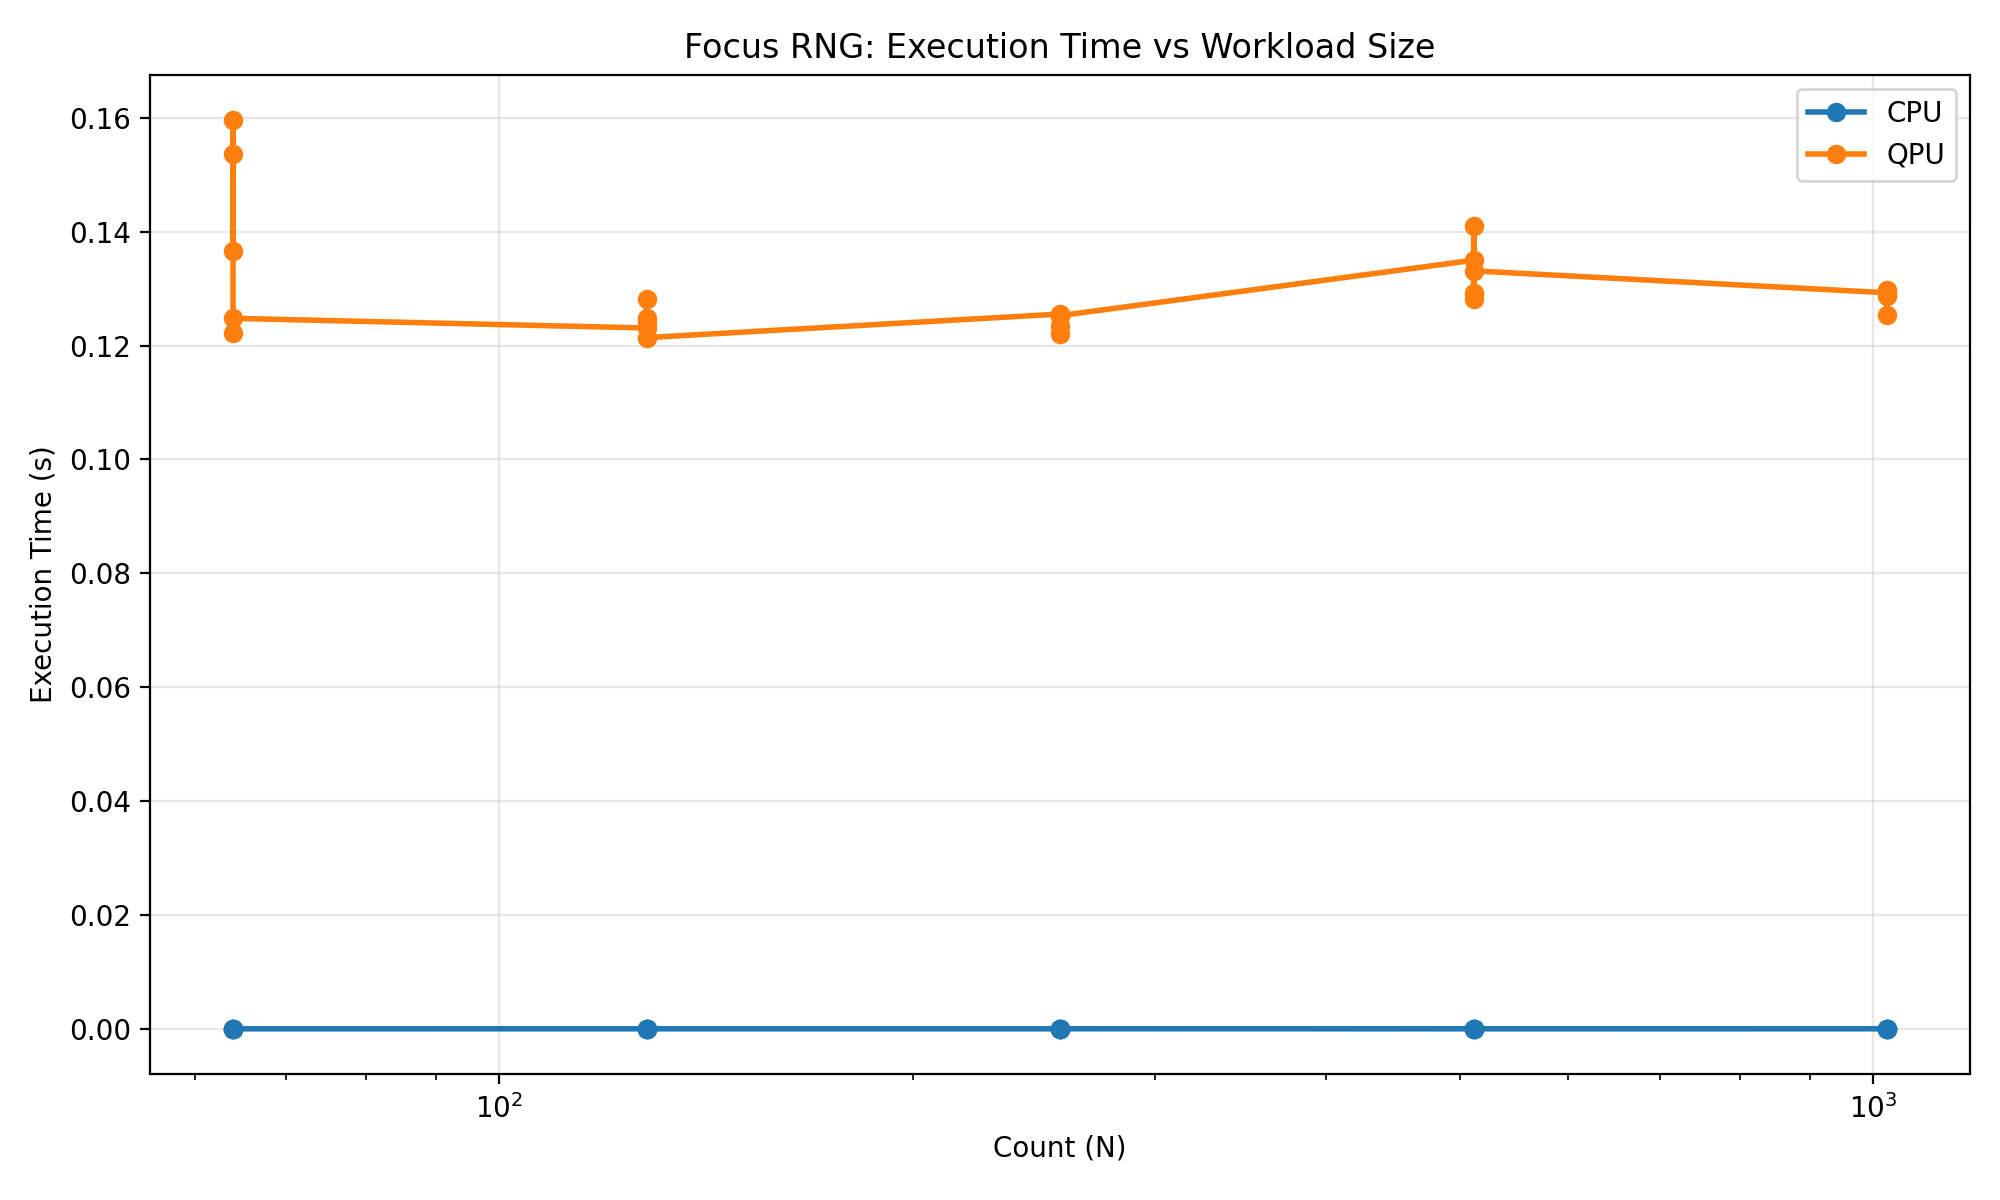
\includegraphics[width=0.98\columnwidth]{figures/fig_execution_time_vs_count_main.png}
  \caption{Execution time versus workload size for analyzed rows.}
  \label{fig:time}
\end{figure}

\begin{figure}[t]
  \centering
  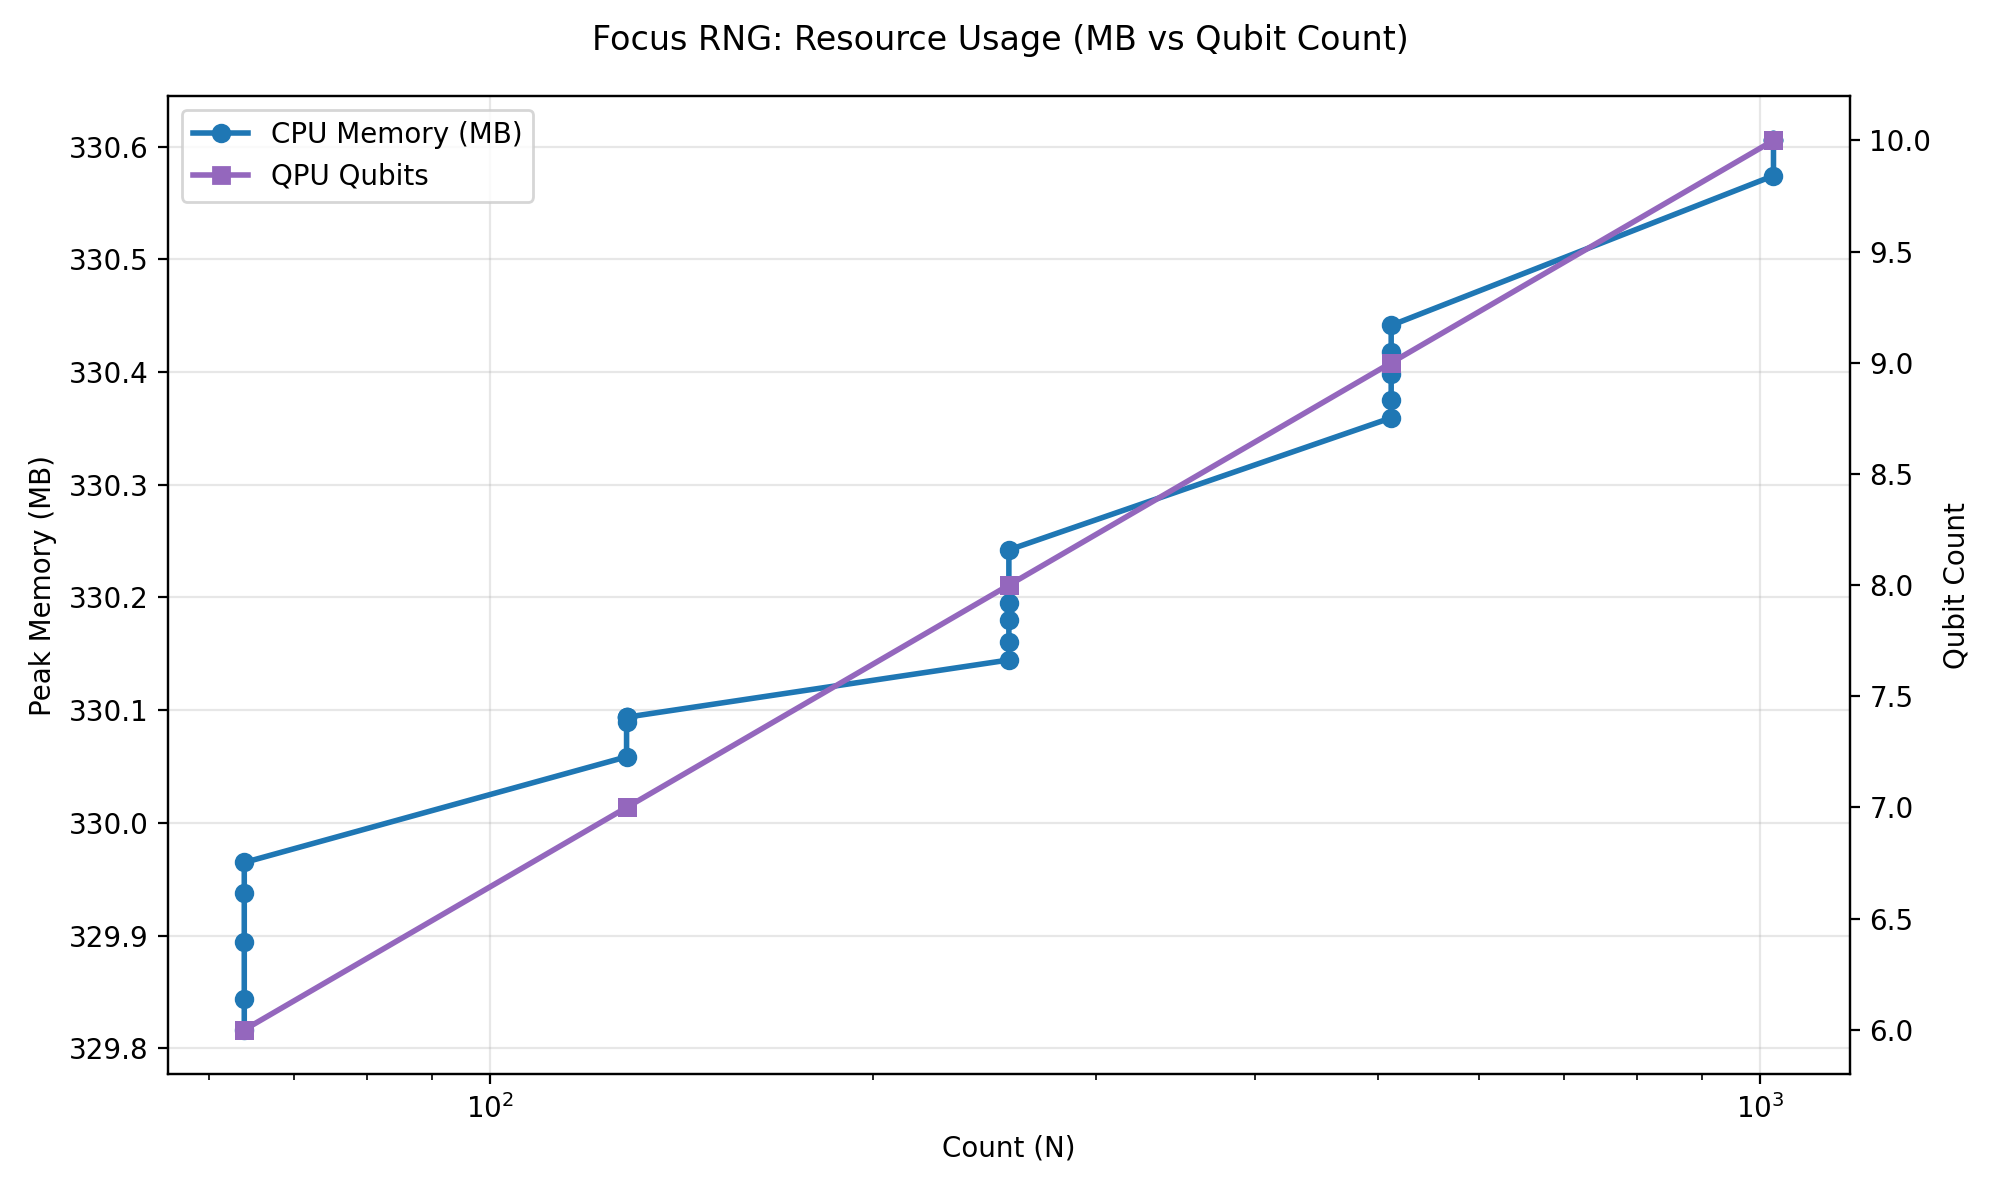
\includegraphics[width=0.98\columnwidth]{figures/fig_resource_efficiency_main.png}
  \caption{Resource view: CPU/GPU memory (MB) and QPU qubit count.}
  \label{fig:resource}
\end{figure}

QPU/CPU speedup values are between $2.77\times10^{-4}$ and $3.34\times10^{-4}$, implying QPU-simulator is approximately three orders of magnitude slower than CPU in this environment.
For CPU-vs-QPU timing comparisons in the primary run, Welch t-tests yield $p < 5\times10^{-5}$ at all tested counts.

\section{Ablations and Error Analysis}
\subsection{Including Fallback Rows}
When fallback rows are included, apparent GPU speedups become 1.09x--1.72x, despite no CUDA execution. Figure~\ref{fig:fallback} shows this confound.

\begin{figure}[t]
  \centering
  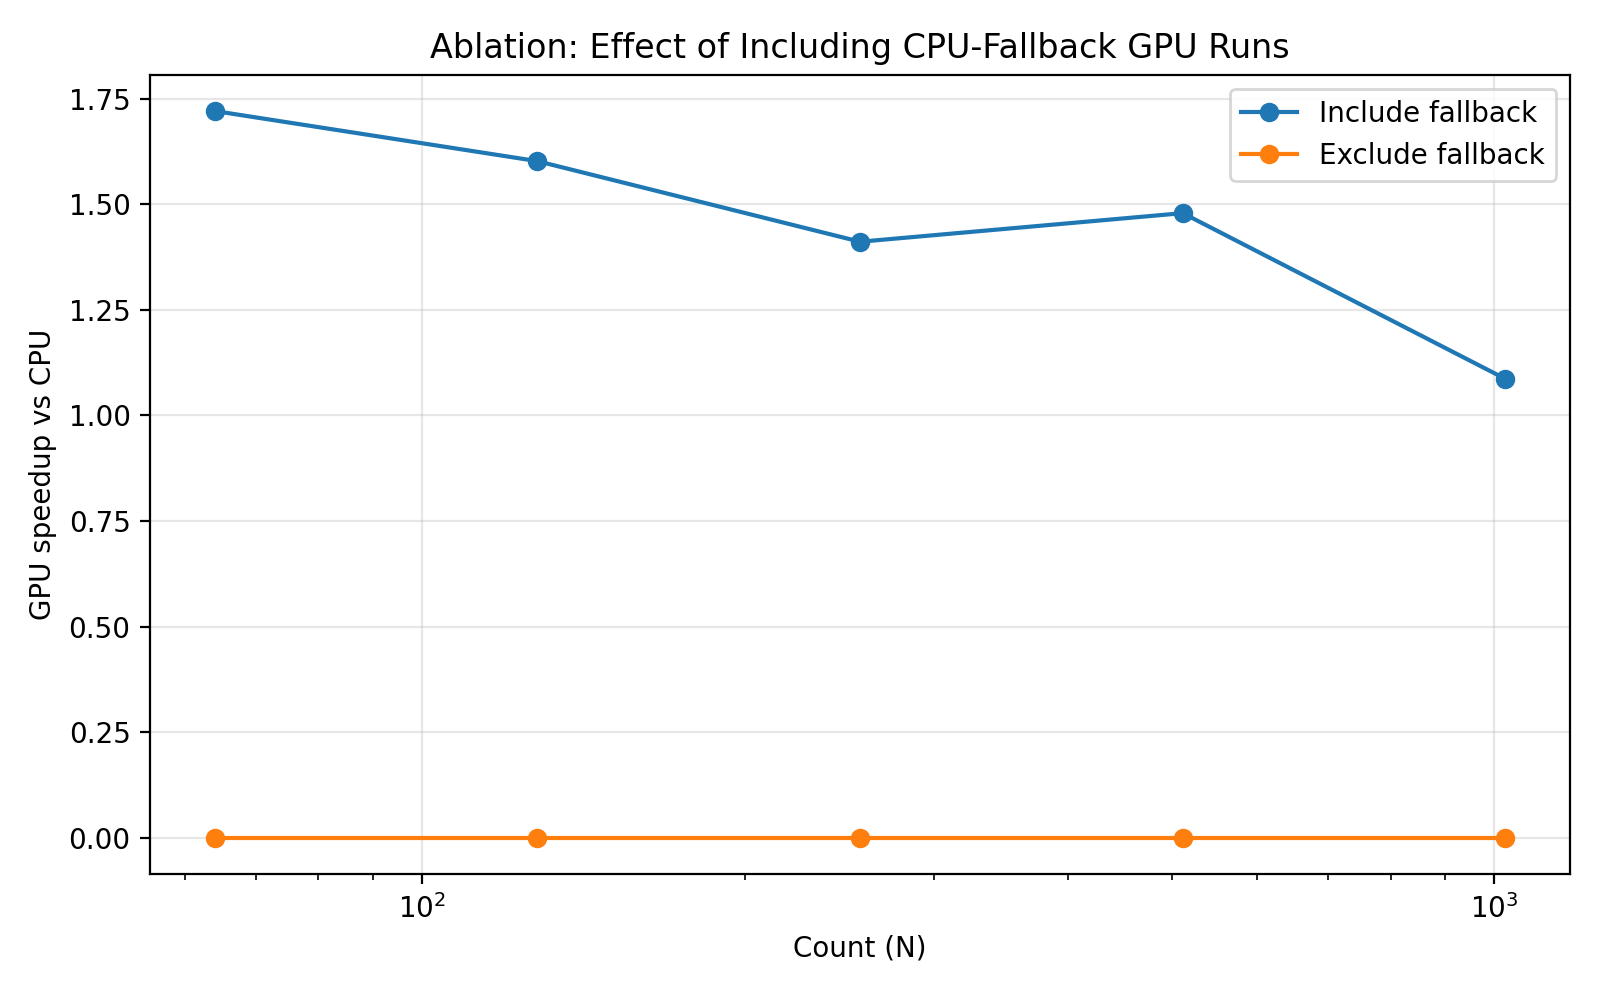
\includegraphics[width=0.98\columnwidth]{figures/fig_ablation_fallback_effect.png}
  \caption{Ablation: including fallback rows changes GPU speedup interpretation.}
  \label{fig:fallback}
\end{figure}

\subsection{Qubit Policy}
Comparing \texttt{logn} and \texttt{fixed} qubit modes changes mean qubits/log2(N) ratio from 1.0 to 1.291, while simulator runtime remains similar in this test range.

\begin{figure}[t]
  \centering
  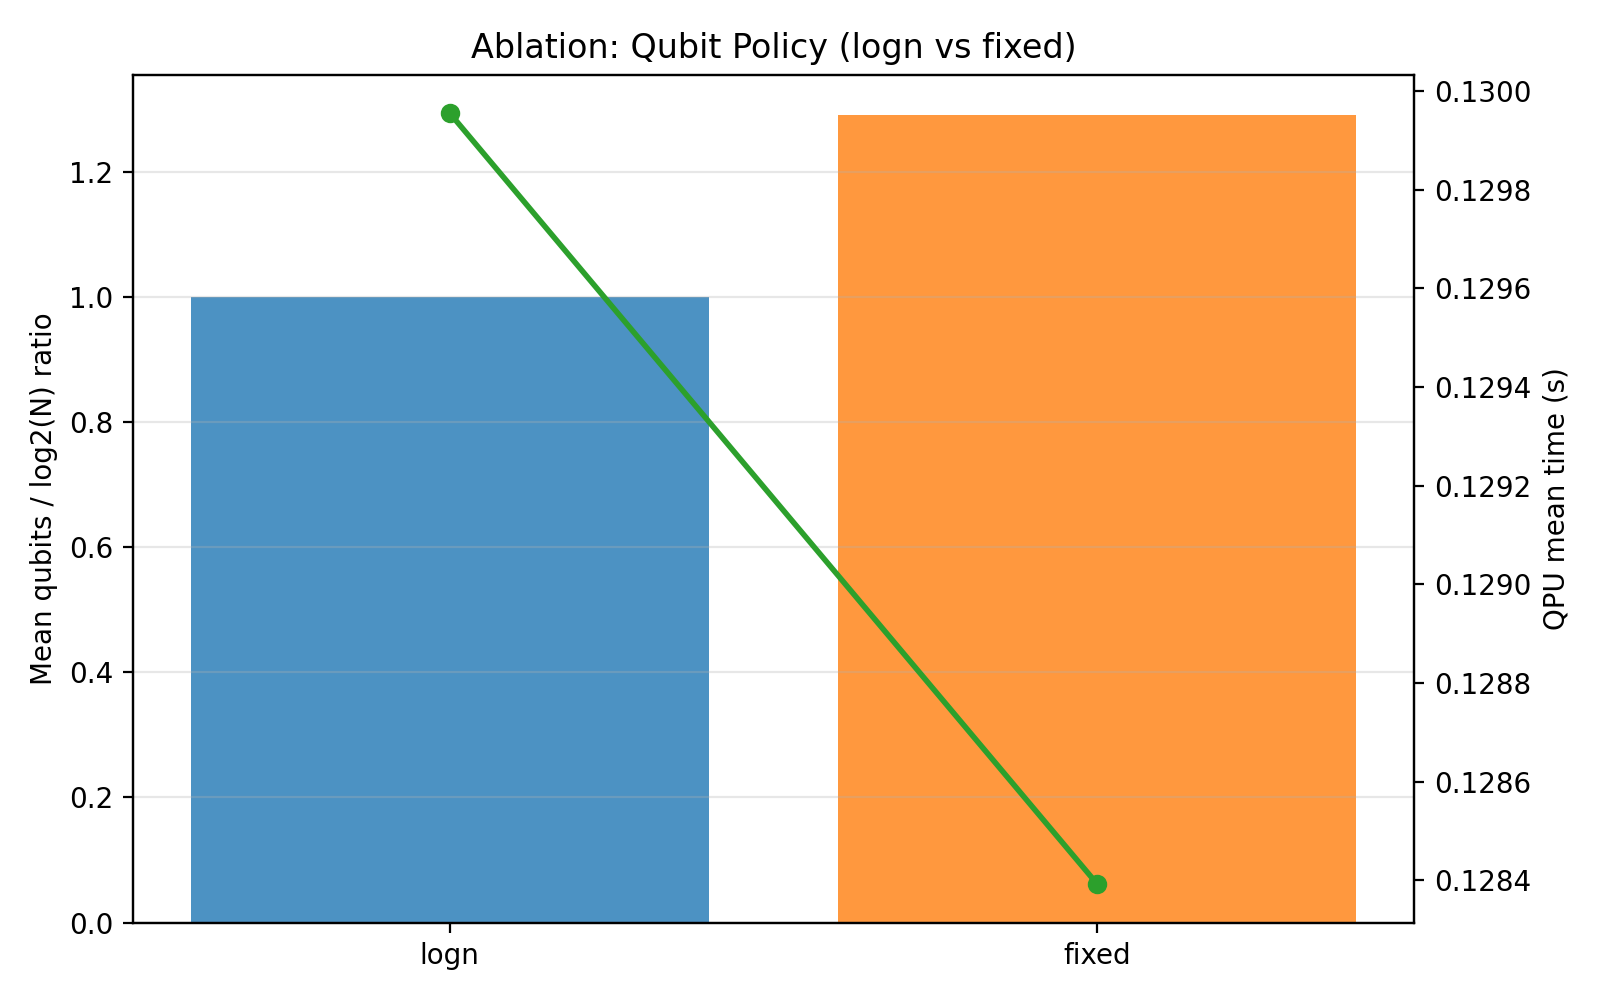
\includegraphics[width=0.98\columnwidth]{figures/fig_ablation_qubit_mode.png}
  \caption{Ablation: qubit policy effect.}
  \label{fig:qmode}
\end{figure}

\subsection{Negative Result}
Historical artifact \texttt{results/reports/focus\_rng\_20260324\_024923} contains QPU failures due to missing \texttt{qiskit} dependency (0/4 QPU success). This is retained as failure evidence, not as performance evidence.

\section{Limitations, Ethics, and Risks}
\begin{itemize}
\item No true CUDA run in current environment.
\item QPU path is simulator-only in reported primary results.
\item Randomness-quality analysis is limited; cryptographic-strength claims are unsupported.
\item MB and qubit metrics are not physically commensurate.
\item Legacy documentation includes energy claims not implemented in current code path.
\end{itemize}

Explicit unsupported claims:
\begin{itemize}
\item Real GPU acceleration over CPU: \textbf{Not supported by current repository evidence}.
\item Real QPU hardware advantage: \textbf{Not supported by current repository evidence}.
\item Certified cryptographic randomness of outputs: \textbf{Not supported by current repository evidence}.
\end{itemize}

\section{Reproducibility}
Primary command:
\begin{verbatim}
MPLCONFIGDIR=/tmp/mpl .venv/bin/python focus_rng_benchmark.py \
  --counts 64,128,256,512,1024 --qubit-mode logn \
  --shots 1024 --warmup 2 --repeats 5 \
  --output-dir results/reports/paper_main
\end{verbatim}

Traceability is documented in \texttt{paper/traceability-matrix.md}; artifact evaluation steps are documented in \texttt{paper/artifact-evaluation.md}.

\section{Conclusion}
The repository provides a useful and reproducible framework for CPU/GPU/QPU RNG benchmarking with explicit fallback handling. In the present environment, conclusions are constrained to CPU and QPU-simulator comparisons. Stronger claims require true CUDA runs, real quantum hardware runs, and stronger randomness-quality evaluation.

\bibliographystyle{IEEEtran}
\bibliography{references}

\end{document}
